\documentclass[11pt]{article}
\usepackage[margin=1in]{geometry}
\usepackage{booktabs,graphicx,amsmath,hyperref,xcolor}
\hypersetup{colorlinks=true,linkcolor=blue,urlcolor=blue,citecolor=blue}
\title{Agentic Weight-Space Programming of a 2B Language Model:\\GPT-6.2 Sol Edits Qwen3.5-2B for SVG Generation}
\author{Experiment run with the Devin/Cognition harness\\\small\url{https://github.com/dylanler/weight-space-programming-experiment}}
\date{November 2026}
\begin{document}
\maketitle

\begin{abstract}
We test whether a frontier coding agent can do \emph{weight-space programming}: improve a language model by reading and editing its weights directly, with no gradient-based training. The agent is GPT-6.2 Sol running in the Devin harness, and the model is \texttt{Qwen/Qwen3.5-2B}, evaluated on five SVG-drawing tasks with countable constraints.
The agent had a live, authenticated Python kernel on one A100 and only development prompts. In about 42 minutes and 5 generation batches it produced a two-round rank-1 projection edit. The edit touches $1{,}370{,}750$ weights ($0.073\%$), all in five MLP \texttt{down\_proj} matrices.
We rendered 500 held-out test outputs to PNG and had independent image-only LLM judges score them. Correct outputs rose from 88/500 to 147/500 (exact McNemar $p<10^{-6}$). A blinded paired re-judging, in which one judge scored base and edited images mixed together, gives 78 vs.\ 120 ($p\approx10^{-6}$).
The edit almost eliminates degenerate repetition loops: generations hitting the 4096-token cap fell from 76 to 6. Correctness improved on three tasks (apple tree, bar chart, circle grid). It did not improve on the two tasks that need joint exact counting (buildings, flags).
\end{abstract}

\section{Introduction}
Weight-space programming~\cite{wsp} treats a network's parameters as editable code: an agent inspects activations and weights, forms mechanistic hypotheses, and writes targeted tensor edits instead of training. We ask two questions. Is the approach \emph{effective} for an autonomous agent, meaning it improves held-out task performance? Is it \emph{efficient}, meaning the edits are small and cheap to find?
We study a small (2B) open model on visual-program-synthesis tasks whose correctness can only be judged by looking at the rendered output.

\section{Experimental setup}
\paragraph{Model and inference.} \texttt{Qwen/Qwen3.5-2B} (24 layers; hidden size 2048; a mix of Gated DeltaNet and full-attention layers) is served with vLLM on a Modal A100-40GB. Decoding is greedy, in non-thinking chat mode, with at most 4096 new tokens. All functions scale to zero when idle.
\paragraph{Tasks.} There are five task families, each with 100 seeded random test prompts and a separate set of 30 dev prompts drawn with a different seed (Table~\ref{tab:tasks}). Every prompt ends with ``Output only the complete SVG code''.
\begin{table}[h]\centering\small
\begin{tabular}{ll}\toprule
Task & Requirement (random parameters)\\\midrule
building & exactly $X$ windows in total and exactly $Y$ floors ($X\in[1,24],Y\in[1,8]$)\\
apple\_tree & a tree with exactly $N$ red apples ($N\in[1,15]$)\\
circle\_grid & a grid of circles with $R$ rows and $C$ columns ($R,C\in[1,6]$)\\
bar\_chart & $N$ bars; the $k$-th is tallest and red, others blue ($N\in[3,9]$)\\
flag & exactly $S$ horizontal stripes and $M$ stars ($S\in[2,9],M\in[1,9]$)\\\bottomrule
\end{tabular}\caption{SVG task families.}\label{tab:tasks}\end{table}

\paragraph{Image-only verification.} The first \texttt{<svg>\ldots</svg>} block in each output is rendered to a 512\,px PNG with CairoSVG. An output with no renderable SVG is incorrect. Judges are separate GPT-6.2 Sol sessions that receive only PNGs and the natural-language requirement. They never see SVG source or model identity, and item IDs are salted hashes. They are told to judge visually and strictly, without programmatic pixel analysis.
We use two protocols: (i) \emph{independent}, where fresh judges score each condition and task separately (100 images per judge), and (ii) \emph{paired-blind}, where base and edited images for a task are shuffled together and scored by a single judge (200 images).

\paragraph{Editing environment.} The editor is a GPT-6.2 Sol session given the reference post~\cite{wsp}, the task descriptions, and an HTTP API to a stateful kernel that holds the vLLM model in eager mode on an A100. The API offers arbitrary Python execution against the live model (weights and temporary forward hooks), a dev-set evaluation endpoint that returns rendered PNGs, and patch saving.
Constraints: no gradient training, fine-tuning, LoRA training, prompt changes, or decoding changes, and a budget of 40 generation batches. The editor never had access to test prompts or test judgments. The saved sparse patch is applied to fresh base weights in a separate function to generate the test outputs.

\section{The edit found by the agent}
The agent first diagnosed the failures. Many base outputs never terminate: they repeat SVG elements until they hit the token cap (48\% for apple\_tree and 23\% for building on test). Using teacher-forced replays of dev generations, it labelled tokens after loop onset as \emph{loop} and tokens of finished generations as \emph{normal}.
At element-boundary positions, where the model chooses between opening another element and closing, it computed a per-layer unit direction $u_\ell \propto \bar h^{\text{loop}}_\ell-\bar h^{\text{normal}}_\ell$. The separation grows with depth, so it targeted odd layers $\ell\in\{15,17,19,21,23\}$.
In each of these layers it selected the top-$k$ MLP neurons by how strongly their output column writes along $u_\ell$, weighted by activation, and applied
\begin{equation}
W^{\text{down}}_{\ell}[:,\mathcal I]\leftarrow \left(I-u_\ell u_\ell^\top\right)W^{\text{down}}_{\ell}[:,\mathcal I].
\end{equation}
Round 1 used $k=128$. Round 2 recomputed the direction on loops that survived round 1 (cosine $0.19$ with round 1 at layer 23) and used $k=32$.
Five variants were evaluated on dev (Table~\ref{tab:dev}). Before each generation batch, the agent screened candidates with teacher-forced checks; for the final edit, normal-text NLL went from 0.058 to 0.061 and greedy agreement from 0.989 to 0.987.
\begin{table}[h]\centering\small
\begin{tabular}{llrrr}\toprule
Edit & Description & \#weights & Rendered & Correct\\\midrule
base & -- & 0 & 124/150 & 27/150\\
E1 & round 1, L15--21, top-64 & 503{,}134 & 140 & 31\\
E2 & round 1, L15--23, top-128 & 1{,}253{,}339 & 144 & 44\\
E3 & round 1, L11--23, top-128 & 1{,}752{,}892 & 143 & 35\\
E4 & E2 + round 2, top-64 & 1{,}622{,}668 & 146 & 39\\
\textbf{E5} & E2 + round 2, top-32 & \textbf{1{,}370{,}750} & \textbf{150} & \textbf{46}\\\bottomrule
\end{tabular}\caption{Editor's dev-set results (correctness judged by the editor itself from PNGs).}\label{tab:dev}\end{table}

\section{Results}
\begin{table}[h]\centering\small
\begin{tabular}{lrrrrrrr}\toprule
Task & \multicolumn{2}{c}{Rendered} & \multicolumn{2}{c}{Visually correct} & $\Delta$ & Fixed & Broken\\
& base & edit & base & edit & & & \\\midrule
Building (windows, floors) & 77 & 99 & 4/100 & 2/100 & -2 & 2 & 4 \\
Apple tree (apples) & 52 & 98 & 11/100 & 33/100 & +22 & 28 & 6 \\
Circle grid (rows, cols) & 100 & 100 & 38/100 & 58/100 & +20 & 23 & 3 \\
Bar chart (n, tallest) & 100 & 100 & 35/100 & 54/100 & +19 & 22 & 3 \\
Flag (stripes, stars) & 95 & 97 & 0/100 & 0/100 & +0 & 0 & 0 \\
\midrule
\textbf{Total} & 424 & 494 & 88/500 & 147/500 & +59 & 75 & 16 \\
\bottomrule\end{tabular}

\caption{Held-out test results (100 prompts per task), independent image-only judges. Fixed/broken count prompts that flipped between incorrect and correct.}\label{tab:main}\end{table}

\begin{figure}[h]\centering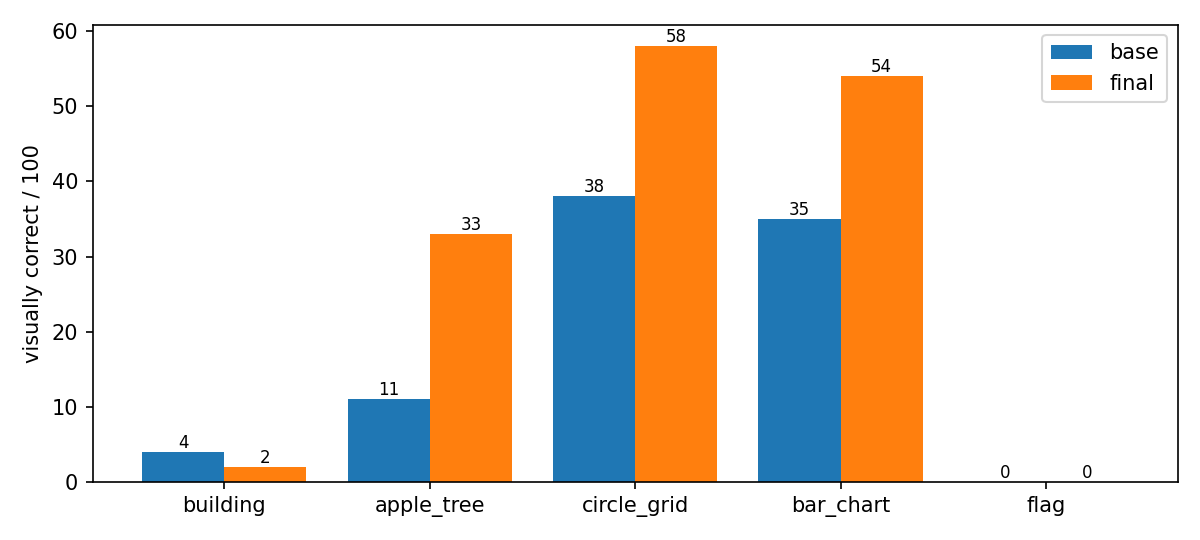
\includegraphics[width=.85\linewidth]{figs/scores.png}\caption{Visually correct outputs per task (independent judges).}\end{figure}

\begin{table}[h]\centering\small
\begin{tabular}{lrrrrr}\toprule
Task & Base & Edit & $\Delta$ & Fixed/Broken & McNemar $p$\\\midrule
building & 5 & 4 & $-1$ & 3/4 & 1.0\\
apple\_tree & 12 & 33 & $+21$ & 27/6 & $3\times10^{-4}$\\
circle\_grid & 21 & 29 & $+8$ & 10/2 & 0.039\\
bar\_chart & 40 & 54 & $+14$ & 18/4 & 0.004\\
flag & 0 & 0 & 0 & 0/0 & --\\\midrule
Total & 78 & 120 & $+42$ & 58/16 & $1\times10^{-6}$\\\bottomrule
\end{tabular}\caption{Paired-blind judging: one judge per task scores 200 shuffled base and edited images.}\label{tab:paired}\end{table}

Under the independent protocol, McNemar tests per task give $p\approx2\times10^{-4}$ (apple\_tree), $9\times10^{-5}$ (circle\_grid), $2\times10^{-4}$ (bar\_chart), 0.69 (building), and $<10^{-6}$ in total.
Generations hitting the length cap fell from 76 to 6, renderable outputs rose from 424 to 494, and total generated tokens fell from 648k to 403k ($-38\%$).

\paragraph{Judge reliability.} Over the 918 rendered images scored by both protocols, the judges agree 93.6\% of the time (Cohen's $\kappa=0.82$). Per task, $\kappa$ is $0.98$ (apple\_tree), $0.91$ (bar\_chart), $1.0$ (flag), $0.79$ (building), and only $0.53$ for circle\_grid, where judges differed on whether partly clipped circles count. The size of the circle-grid gain therefore depends on the judge ($+20$ vs.\ $+8$), but it is significant under both protocols.

\section{Discussion}
\paragraph{Effectiveness.} The agent found a genuine mechanism, a late-layer residual direction that sustains repetition at element boundaries, and removed it with an interpretable low-rank edit. The improvement transferred from 150 dev prompts to 500 unseen test prompts.
Part of the gain is mechanical: outputs that used to loop now render, which drives most of the apple-tree improvement. Bar chart and circle grid improved even though their render rates were unchanged (100/100 for both models), which suggests that suppressing repetition also reduces over-generated duplicate elements.
The edit did \emph{not} improve compositional counting. Buildings with exact windows and floors stay at 2--5\%, and flags at 0\%; the model rarely draws recognizable stars. The agent stated this limitation itself.
\paragraph{Efficiency.} The edit took about 42 minutes of agent wall-clock time and 5 of 40 generation batches, with no backpropagation. It changes 0.073\% of parameters in five matrices, and a short script reproduces it exactly from the base weights.
\paragraph{Limitations.} The judges are LLMs rather than humans. We used a single seed and greedy decoding. The editor selected among edits using its own dev-set judgments. The agents' model identity is the organization default (GPT-6.2 Sol, Preview) and was not verified per call.

\section{Conclusion}
Within an hour, using a small fraction of its evaluation budget, an agentic GPT-6.2 Sol performed useful weight-space programming on Qwen3.5-2B. It found and surgically removed a repetition mechanism, improving held-out visual correctness from 88 to 147 of 500 (or 78 to 120 under stricter blinded paired judging).
Weight-space programming was effective here for a pathology with a clean linear signature. It was not effective for the skill-level deficit of exact compositional counting, which remains open for future agents.

\begin{thebibliography}{1}
\bibitem{wsp} Weight-Space Programming (blog post). \url{https://rikiyat.github.io/blog/weight-space-programming/}.
\end{thebibliography}
\end{document}
